\chapter{Printing Your Thesis}
\label{cha:Printing}


\section{PDF Workflow}
\label{sec:pdf-workflow}

Nowadays \latex\ is practically always used in such a way that it creates PDF
documents directly (without the detour via DVI and PostScript that was common
in the past). In modern environments (\eg, \emph{TeXstudio} or \emph{Overleaf})
this works automatically without any further configuration effort.


\subsection{PDF Archive Format (PDF/A)}
\label{sec:PDFA}

Many institutions require theses to be submitted in PDF/A format, which is a
standardized variant of PDF for archiving and long-term preservation.%
\footnote{\url{https://en.wikipedia.org/wiki/PDF/A}}
This document is rendered in PDF/A format by default (PDF/A-2b to be exact),
caused by
%
\begin{LaTeXCode}[numbers=none]
\RequirePackage{hgbpdfa}
\end{LaTeXCode}
%
at the beginning of file \verb!main.tex! (loading \verb!hgbpdfa.sty!).
Note that this must be placed \emph{before} the \verb!\documentclass!
declaration. Required meta-data (\eg, author and title) are automatically 
derived from the document settings and inserted into the output PDF.%
\footnote{This setup builds on new functionality currently being added to
the \texttt{pdflatex} kernel and requires package \texttt{pdfmanagement-testphase}
version 0.95s (2022-09-26) or higher. With older versions, a package warning is
issued and no PDF/A is produced.}


\subsection{PDF/A Issues}
\label{sec:PDFA-issues}

Activating the PDF/A option creates an output file that \emph{claims} to be 
PDF/A-compliant but this does not imply that is actually \emph{is}.
Although \emph{this} document produces a compliant PDF/A, any derived document
may not do so. It is therefore important to \emph{validate} the resulting PDF file
before submission using one of the options described below. Most violations
of the PDF/A standard arise from the inclusion of other PDF files, particularly 
graphics. Typical issues are related to the use of non-embedded fonts
and incorrect or unwanted color spaces. This setup assumes sRGB colors, 
which should also be used when creating your own illustrations.

Problems with imported PDF files may be difficult to locate in the final (composite)
document. Once the troubling file is known and cannot be regenerated, it may be fixed using 
other tools such as Adobe \emph{Acrobat} (\emph{Distiller}) or \emph{Ghostscript}.%
\footnote{\url{https://ghostscript.com/}}


\subsection{PDF/A Validation}
\label{sec:PDFA-validation}

A straightforward (and free) method to validate PDF/A compliance is provided by
\textsf{veraPDF}, which includes
%
\begin{itemize}
\item an open-source validation client%
  \footnote{\url{https://verapdf.org/software} (Windows, macOS, Linux)} and
\item an online validation service.%
  \footnote{\url{https://demo.verapdf.org}}
\end{itemize}
%
See Figure \ref{fig:verapdf-report} for an example.
A similar service is offered by \textsf{pdf-online.com},%
\footnote{\url{https://www.pdf-online.com/osa/validate.aspx}}
unfortunately announced to be retired in the near future.
Of course, PDF/A validation is also contained in the toolset of Adobe \emph{Acrobat}.

\begin{figure}[htbp]
    \centering
    \fbox{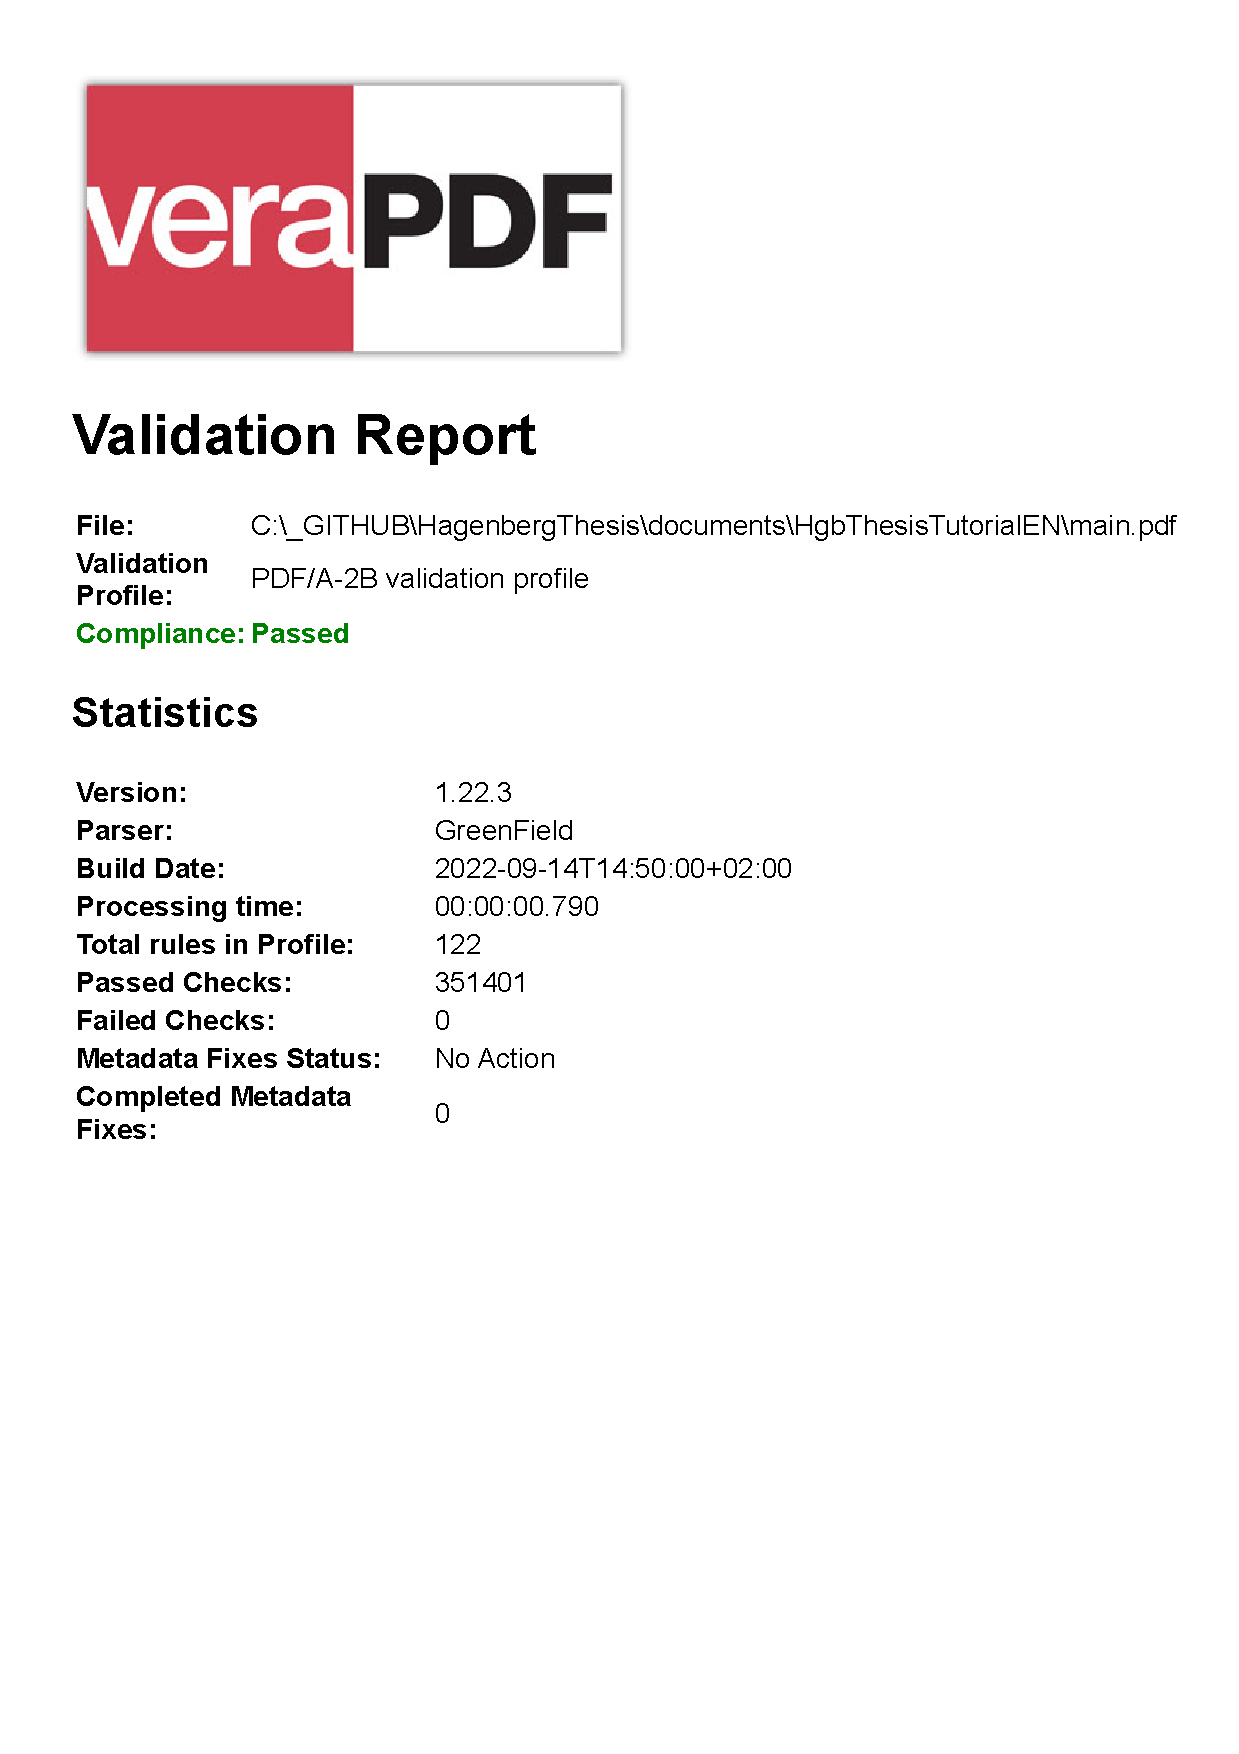
\includegraphics[width=.60\textwidth]{verapdf-report}}
    \caption{Report produced by the \textsf{veraPDF} client after successful validation
    of \emph{this} document. Note that this screenshot was imported as a PDF 
    which itself is \emph{not} PDF/A-compliant.}
    \label{fig:verapdf-report}
\end{figure}


\section{Printing}

Before printing the manuscript, it is advisable to consider a few things in
order to avoid unnecessary trouble (and costs).

\subsection{Digital Submission versus Printing}

For reasons of sustainability, many degree programs no longer require printed
submissions, especially for bachelor's theses. In this case, uploading a PDF
file is sufficient. The declaration is then either signed digitally in the
document or obtained in another way by the degree program. It is advisable to
find out the submission requirements in good time to avoid unnecessary printing
of one's work.

\subsection{Printer and Paper}

If the thesis is printed, this must be done for the final version on a
high-quality \emph{laser printer}; printouts made with inkjet printers are
\emph{not} sufficient. The paper used should also be of good quality (woodfree)
and usual grammage (typ.\ $80\,\mathrm{g} / \mathrm{m}^2$). If only a few
\emph{color} pages are necessary, one may print them separately on a color laser
printer and insert them into the main document (printed in black and white).

By the way, \emph{all} copies to be handed in should be \emph{printed} (and not 
copied)! The cost of printing is no higher than that of copies, but the difference
in quality is---especially for pictures and graphics---usually significant.


\subsection{Print Size}

First of all, make sure that the paper size set in the final PDF file is really
\textrm{A4}! This can be done, for example, with Adobe \emph{Acrobat} or 
\emph{SumatraPDF} via \texttt{File} $\rightarrow$ \texttt{Properties} 
to show the document's paper size:
%
\begin{center}
	\textrm{Correct:} A4 = $8{,}27 \times 11{,}69$ inches or $210 \times 297$ mm.
\end{center}
%
If this does not match, then probably "Letter" is set as the paper size somewhere
in the workflow by mistake.

A common and easily overlooked error when printing PDF documents is caused by 
accidentally setting the "Fit to page" option in the print menu, usually printing 
pages that are too small. Therefore, make sure you check the size of the printout 
by verifying the text width%
\footnote{\Convert[unit=mm]{\the\textwidth}	in this document.} % using 'lengthconvert' package
or using the measurement frame included at the end of this document.
To be on the safe side, this measurement frame should be kept until the work 
is completed, and only then the corresponding page should be removed.
If, as mentioned before, individual color pages are printed separately, these 
should of course also be checked carefully for compliance with the print size!